\section{Описание модуля}
Модуль \verb"geometry" представляет из себя подключаемый пакет на языке {\sf C++}. Состоит из двух файлов \verb"geometry.hpp" и \verb"geometry.cpp". В модуле реализован набор классов, отвечающих за базовые пространственные фигуры (примитивы), преобразование фигур (сдвиг, поворот, трансформация) и алгебры битовых операций для комбинирования нескольких фигур (объединение, пересечение, исключение). Модуль использует в качестве подключаемого пакета библиотеку {\sf aivlib}. Проекты с подключенным модулем можно также компилировать с использованием {\sf SWIG~2}.

\begin{wrapfigure}{r}{250pt}
    \begin{center}
        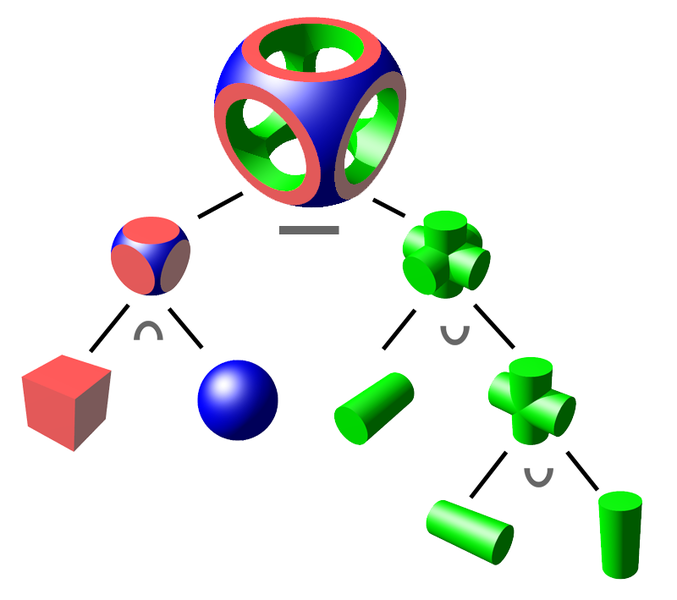
\includegraphics[width=7cm]{images/Csg_tree.png}
    \end{center}
    \caption{Сложный объект может быть представлен двоичным деревом, где «листья» — это объекты, а узлы — операции. ($\cap$~--- пересечение, $\cup$~--- объединение, ---~--- разность)}
    \label{img:csg}
\end{wrapfigure}
В основе пакета лежит технология <<Конструктивная сплошная геометрия>> (Constructive Solid Geometry, CSG)~\cite{csg}. Характерный пример использования этой технологии изображен на рис.~\ref{img:csg}.


Все классы объектов являются наследниками базового типа \verb"BaseFigure". Из наследников класса набирается древовидное дерево выражения, листьями которго являются примитивы, а остальные вершины либо объекты преобразований либо объекты битовых операций. Для контроля за указателями использован прокси-класс \verb"Figure", с "умным" указателем в \verb"private" поле \verb"std::shared_ptr<BaseFigure> figure". 

У каждого класса фигуры определены два метода~--- \verb"get_min()" и \verb"get_max()", которые возвращают координаты левого нижнего и правого верхнего угла вмещающего прямоугольного параллелепипида(bounding box). При преобразовании фигур и при битовых операциях bounding box вычисляется относительно детей.

\section{Примитвы}
Примитивы~---основы для набора сложных фингур. Для создания экземпляров прокси-класса для примитивов используются порождающие глобальные функции.

\subsection{Сфера}
Создается порождающей глобальной функцией
\begin{verbatim}
Figure spheroid(const aiv::vctr<3> center, double R);
\end{verbatim}
, где \verb"center"~--- центр сферы, \verb"R"~--- радиус сферы.

\subsection{Цилиндр}
Создается порождающей глобальной функцией
\begin{verbatim}
Figure cylinder(const aiv::vctr<3> bottom_origin_center, const aiv::vctr<3> &n, 
    double R, double H);
\end{verbatim}
, где \verb"bottom_origin_center"~--- центр нижнего основания цилиндра, \verb"n"~--- направляющаяя, выходящяя из нижнего основания в сторону верхнего, перпендикулярно нижнему основанию, \verb"R"~---радиус оснований, \verb"H"~--- высота цилиндра.

\subsection{Прямоугольный параллелепипид}
Создается порождающей глобальной функцией
\begin{verbatim}
Figure box(const aiv::vctr<3> bottom_origin_center, const aiv::vctr<3> &n, 
    double phi, double A, double B, double H);
\end{verbatim}
, где \verb"bottom_origin_center"~--- центр нижней грани, \verb"n"~--- направляющаяя, выходящяя из нижней грани в сторону верхней, перпендикулярно нижней грани, \verb"phi"~--- угол поворота вокруг линии, соединяющей центры нижней и верхней граней по часовой стрелке, \verb"A",\verb"B",\verb"C"~--- длина ребер вдоль осей X,Y,Z соответственно.

\subsection{Куб}
И функцией
\begin{verbatim}
Figure cube(const aiv::vctr<3> bottom_origin_center, const aiv::vctr<3> &n, 
    double phi, double A);
\end{verbatim}
, где \verb"bottom_origin_center"~--- центр нижней грани, \verb"n"~--- направляющаяя, выходящяя из нижней грани в сторону верхней, перпендикулярно нижней грани, \verb"phi"~--- угол поворота вокруг линии, соединяющей центры нижней и верхней граней по часовой стрелке, \verb"A"~--- длина ребра куба.

\section{Преобразование фигур}
Преобразования фигур реализованы как методы класса \verb"Figure", возвращающие экземпляры класса \verb"Figure". 

\subsection{Сдвиг}
\begin{verbatim}
Figure Figure::move(const aiv::vctr<3> &offset);
\end{verbatim}
, где \verb"offset"~--- смещение фигуры.

\subsection{Поворот вокруг прямой по часовой стрелке}
\begin{verbatim}
Figure Figure::rotate(const aiv::vctr<3> &center, const aiv::vctr<3> &n_phi);
\end{verbatim}
, где \verb"center"~--- точка, из которой будет выходит образующая прямой, вокруг которой поворачиваем, \verb"n_phi"~--- направление образующей прямой, вокруг которой поворачиваем, а длина вектора \verb"n_phi" равна углу, на который поворачиваем.
\subsection{Трансформация}
\begin{verbatim}
Figure Figure::transform(const aiv::vctr<3> &center, const aiv::vctr<3> &ox, 
    const aiv::vctr<3> &oy, const aiv::vctr<3> &oz);
\end{verbatim}
, где \verb"center"~--- центр новой системы координат в координатах старой,\verb"ox", \verb"oy", \verb"oz"~--- новые оси координат, выраженные в координатах старой системы.

\section{Алгебра битовых операций}
Битовые операции над фигурами исполнены при помощи перегрузки операторов сложения, умножения и вычитания для экземпляров класс \verb"Figure".
Нужно быть внимательным и правильно расставлять скобки, так как битовых операциях не всегда выполняется коммутативность.
\begin{itemize}
    \item Объединение~--- перегруженный оператор сложения ($+$)
    \item Пересечение~--- перегруженный оператор умножения ($*$)
    \item Исключение~--- перегруженный оператор вычитания ($-$)
\end{itemize}

\section{Пример использования}
\subsection{C++}
\begin{verbatim}
#include "geometry.hpp"
using namespace aiv;
int main(){
   Figure f1 = cylinder(Vctr(0.,0.,0.),Vctr(0.,0.,1.), 20., 20.);
   Figure f2 = f1.rotate(Vctr(0.,0.,0.), Vctr(1.,1.,1));
   Figure f3 = f1 + f2;

   vctr<3> my_min = f3.get_min()
   vctr<3> my_max = f3.get_max()

   printf("Результат проверки вхождения вектора Vctr(3., 10., 0.) в 
    фигуру f3 %s", f3.check(Vctr(3., 10., 0.)) ? "true" : "false")
   return 0;
}
\end{verbatim}

\subsection{python}
\begin{verbatim}
from geometry import *
import math
e_fig1 = cube(Vctr(0., 0., 0.), Vctr(0.,0.,1.), 0., 20)
e_fig2 = spheroid(Vctr(0.,0., 10.), 10 * math.sqrt(2)*0.9)
e_fig3 = cylinder(Vctr(0.,0.,0.), Vctr(0., 0., 1.), 6, 20 )
e_fig4 = cylinder(Vctr(-10.,0.,10.), Vctr(1., 0., 0.), 6, 20 )
e_fig5 = cylinder(Vctr(0.,-10.,10.), Vctr(0., 1., 0.), 6, 20 )

final_fig = e_fig1*e_fig2-(e_fig3+e_fig4+e_fig5)
final_fig_1 = e_fig1*e_fig2-(e_fig3+e_fig4+
    e_fig5.move(Vctr(3.,0.,3.)).rotate(Vctr(3.,-11.,3.), Vctr(0.,0.,-0.2)))
\end{verbatim}

\subsection{magnus}
В пакете magnus для моделирования эволюции магнетков модуль \verb"geometry" играет одну из главных ролей. При помощи фигур из этого модуля задается формы области магнитных образцов.
В примере использования на языке {\sf Python} фигура \verb"final_fig" является прототипом фигуры с рисунка~\ref{img:csg}. Если проиницализировать магнитный образей при помощи этой фигуры и вывести его изображение через пакет {\sf MagView}, то получим аналогиную картину (см. рис.~\ref{img:mycsg}).

\begin{figure}
    \begin{center}
        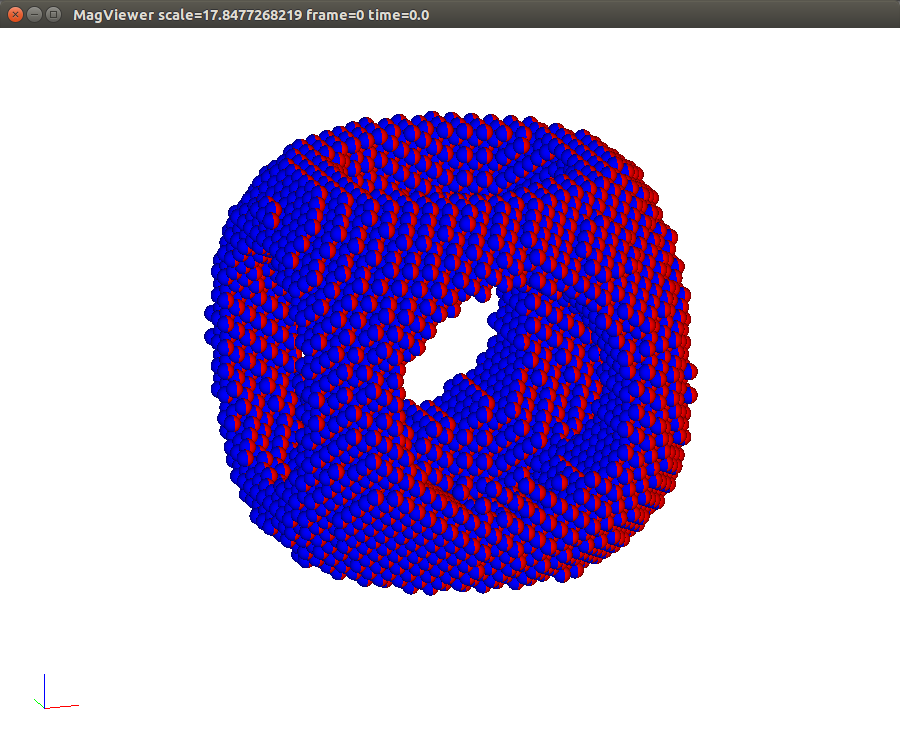
\includegraphics[width=12cm]{images/my_Csg_tree.png}
    \end{center}
    \caption{Полученный магнитный образец с применением модуля}
    \label{img:mycsg}
\end{figure}


\newpage
\begin{thebibliography}{9}
    \bibitem{csg} \textit{Foley, James D.} (1996), "12.7 Constructive Solid Geometry", Computer Graphics: Principles and Practice, Addison-Wesley Professional, pp. 557–558, ISBN 9780201848403.
\end{thebibliography}
